% \iffalse
\let\negmedspace\undefined
\let\negthickspace\undefined
\documentclass[beamer]{IEEEtran}
\usepackage{cite}
\usepackage{amsmath,amssymb,amsfonts,amsthm}
\usepackage{algorithmic}
\usepackage{graphicx}
\usepackage{textcomp}
\usepackage{xcolor}
\usepackage{txfonts}
\usepackage{listings}
\usepackage{enumitem}
\usepackage{mathtools}
\usepackage{gensymb}
\usepackage{comment}
\usepackage[breaklinks=true]{hyperref}
\usepackage{tkz-euclide} 
\usepackage{listings}
\usepackage{gvv}                                        
\def\inputGnumericTable{}                                 
\usepackage[latin1]{inputenc}                                
\usepackage{color}                                            
\usepackage{array}                                            
\usepackage{longtable}                                       
\usepackage{calc}                                             
\usepackage{multirow}                                         
\usepackage{hhline}                                           
\usepackage{ifthen}                                           
\usepackage{lscape}
\usepackage[export]{adjustbox}

\newtheorem{theorem}{Theorem}[section]
\newtheorem{problem}{Problem}
\newtheorem{proposition}{Proposition}[section]
\newtheorem{lemma}{Lemma}[section]
\newtheorem{corollary}[theorem]{Corollary}
\newtheorem{example}{Example}[section]
\newtheorem{definition}[problem]{Definition}
\newcommand{\BEQA}{\begin{eqnarray}}
\newcommand{\EEQA}{\end{eqnarray}}
\newcommand{\define}{\stackrel{\triangle}{=}}
\theoremstyle{remark}
\newtheorem{rem}{Remark}
\begin{document}
\parindent 0px
\bibliographystyle{IEEEtran}

\title{Assignment\\[1ex]11.9.1 - 9}
\author{EE23BTECH11220 - R.V.S.S Varun$^{}$% <-this % stops a space
}
\maketitle
\newpage
\bigskip

\renewcommand{\thefigure}{\theenumi}
\renewcommand{\thetable}{\theenumi}
\section*{Question}
Find $a_{9}$ in the sequence $a_{n}=\brak{-1}^{n-1}n^{3}$ 
\section*{Solution}
\textbf{Given,} 
\begin{align}
x\brak{n}=\brak{-1}^{n-1}\cdot n^{3}\cdot u\brak{n}\\ \text{Subsitute n=9,}\nonumber \\x\brak{9}=729\\
X\brak{z}=\sum_{n=-\infty}^{n=\infty}x\brak{n}\cdot z^{-n}\\
X\brak{z}=\frac{6z^2}{\brak{z^2-1}^{2}}\\
\text{ROC}\implies\{z:|z|<1\}
\end{align} 

\begin{table}[h]
    \centering
    \begin{tabular}{|c|c|}
    \hline
        Symbol &Description \\
        \hline
         x\brak{0}& first term of the sequence\\
         \hline
         x\brak{n}& nth term of the sequence \\
         \hline
         $x\brak{n}\xrightarrow{\mathcal{Z}}X\brak{z}$& $\mathcal{Z}$- transform of x\brak{n} \\
         \hline
    \end{tabular}
    \vspace{10pt}
    \caption{Table of parameters}
    \label{tab:my_label}
\end{table}
\begin{figure}[h]
    \centering
    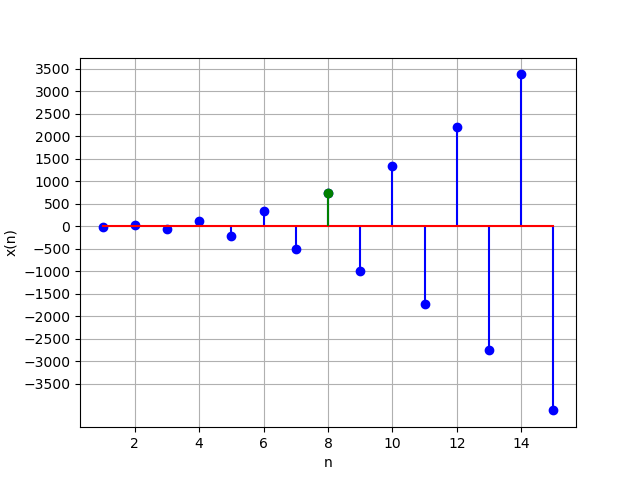
\includegraphics[width=1\linewidth]{graph.png} 
    \label{fig:enter-label}
\end{figure}
\begin{center}
Graph of x\brak{n}
   \end{center}
\end{document}
